\documentclass[ucs, notheorems, handout]{beamer}
\usetheme[numbers,totalnumbers,compress, nologo]{Statmod}
\usefonttheme[onlymath]{serif}
\setbeamertemplate{navigation symbols}{}

\usepackage{graphicx,subcaption,ragged2e}

%new calligraphic font for subspaces 
\usepackage{euscript}
\newcommand{\cA}{\EuScript{A}}
\newcommand{\cB}{\EuScript{B}}
\newcommand{\cC}{\EuScript{C}}
\newcommand{\cD}{\EuScript{D}}
\newcommand{\cE}{\EuScript{E}}
\newcommand{\cF}{\EuScript{F}}
\newcommand{\cG}{\EuScript{G}}
\newcommand{\cH}{\EuScript{H}}
\newcommand{\cI}{\EuScript{I}}
\newcommand{\cJ}{\EuScript{J}}
\newcommand{\cK}{\EuScript{K}}
\newcommand{\cL}{\EuScript{L}}
\newcommand{\cM}{\EuScript{M}}
\newcommand{\cN}{\EuScript{N}}
\newcommand{\cO}{\EuScript{O}}
\newcommand{\cP}{\EuScript{P}}
\newcommand{\cQ}{\EuScript{Q}}
\newcommand{\cR}{\EuScript{R}}
\newcommand{\cS}{\EuScript{S}}
\newcommand{\cT}{\EuScript{T}}
\newcommand{\cU}{\EuScript{U}}
\newcommand{\cV}{\EuScript{V}}
\newcommand{\cW}{\EuScript{W}}
\newcommand{\cX}{\EuScript{X}}
\newcommand{\cY}{\EuScript{Y}}
\newcommand{\cZ}{\EuScript{Z}}

%font for text indices like transposition X^\mathrm{T}
\newcommand{\rmA}{\mathrm{A}}
\newcommand{\rmB}{\mathrm{B}}
\newcommand{\rmC}{\mathrm{C}}
\newcommand{\rmD}{\mathrm{D}}
\newcommand{\rmE}{\mathrm{E}}
\newcommand{\rmF}{\mathrm{F}}
\newcommand{\rmG}{\mathrm{G}}
\newcommand{\rmH}{\mathrm{H}}
\newcommand{\rmI}{\mathrm{I}}
\newcommand{\rmJ}{\mathrm{J}}
\newcommand{\rmK}{\mathrm{K}}
\newcommand{\rmL}{\mathrm{L}}
\newcommand{\rmM}{\mathrm{M}}
\newcommand{\rmN}{\mathrm{N}}
\newcommand{\rmO}{\mathrm{O}}
\newcommand{\rmP}{\mathrm{P}}
\newcommand{\rmQ}{\mathrm{Q}}
\newcommand{\rmR}{\mathrm{R}}
\newcommand{\rmS}{\mathrm{S}}
\newcommand{\rmT}{\mathrm{T}}
\newcommand{\rmU}{\mathrm{U}}
\newcommand{\rmV}{\mathrm{V}}
\newcommand{\rmW}{\mathrm{W}}
\newcommand{\rmX}{\mathrm{X}}
\newcommand{\rmY}{\mathrm{Y}}
\newcommand{\rmZ}{\mathrm{Z}}

%tt font for time series
\newcommand{\tA}{\mathsf{A}}
\newcommand{\tB}{\mathsf{B}}
\newcommand{\tC}{\mathsf{C}}
\newcommand{\tD}{\mathsf{D}}
\newcommand{\tE}{\mathsf{E}}
\newcommand{\tF}{\mathsf{F}}
\newcommand{\tG}{\mathsf{G}}
\newcommand{\tH}{\mathsf{H}}
\newcommand{\tI}{\mathsf{I}}
\newcommand{\tJ}{\mathsf{J}}
\newcommand{\tK}{\mathsf{K}}
\newcommand{\tL}{\mathsf{L}}
\newcommand{\tM}{\mathsf{M}}
\newcommand{\tN}{\mathsf{N}}
\newcommand{\tO}{\mathsf{O}}
\newcommand{\tP}{\mathsf{P}}
\newcommand{\tQ}{\mathsf{Q}}
\newcommand{\tR}{\mathsf{R}}
\newcommand{\tS}{\mathsf{S}}
\newcommand{\tT}{\mathsf{T}}
\newcommand{\tU}{\mathsf{U}}
\newcommand{\tV}{\mathsf{V}}
\newcommand{\tW}{\mathsf{W}}
\newcommand{\tX}{\mathsf{X}}
\newcommand{\tY}{\mathsf{Y}}
\newcommand{\tZ}{\mathsf{Z}}

%bf font for matrices
\newcommand{\bfA}{\mathbf{A}}
\newcommand{\bfB}{\mathbf{B}}
\newcommand{\bfC}{\mathbf{C}}
\newcommand{\bfD}{\mathbf{D}}
\newcommand{\bfE}{\mathbf{E}}
\newcommand{\bfF}{\mathbf{F}}
\newcommand{\bfG}{\mathbf{G}}
\newcommand{\bfH}{\mathbf{H}}
\newcommand{\bfI}{\mathbf{I}}
\newcommand{\bfJ}{\mathbf{J}}
\newcommand{\bfK}{\mathbf{K}}
\newcommand{\bfL}{\mathbf{L}}
\newcommand{\bfM}{\mathbf{M}}
\newcommand{\bfN}{\mathbf{N}}
\newcommand{\bfO}{\mathbf{O}}
\newcommand{\bfP}{\mathbf{P}}
\newcommand{\bfQ}{\mathbf{Q}}
\newcommand{\bfR}{\mathbf{R}}
\newcommand{\bfS}{\mathbf{S}}
\newcommand{\bfT}{\mathbf{T}}
\newcommand{\bfU}{\mathbf{U}}
\newcommand{\bfV}{\mathbf{V}}
\newcommand{\bfW}{\mathbf{W}}
\newcommand{\bfX}{\mathbf{X}}
\newcommand{\bfY}{\mathbf{Y}}
\newcommand{\bfZ}{\mathbf{Z}}

%bb font for standard spaces and expectation
\newcommand{\bbA}{\mathbb{A}}
\newcommand{\bbB}{\mathbb{B}}
\newcommand{\bbC}{\mathbb{C}}
\newcommand{\bbD}{\mathbb{D}}
\newcommand{\bbE}{\mathbb{E}}
\newcommand{\bbF}{\mathbb{F}}
\newcommand{\bbG}{\mathbb{G}}
\newcommand{\bbH}{\mathbb{H}}
\newcommand{\bbI}{\mathbb{I}}
\newcommand{\bbJ}{\mathbb{J}}
\newcommand{\bbK}{\mathbb{K}}
\newcommand{\bbL}{\mathbb{L}}
\newcommand{\bbM}{\mathbb{M}}
\newcommand{\bbN}{\mathbb{N}}
\newcommand{\bbO}{\mathbb{O}}
\newcommand{\bbP}{\mathbb{P}}
\newcommand{\bbQ}{\mathbb{Q}}
\newcommand{\bbR}{\mathbb{R}}
\newcommand{\bbS}{\mathbb{S}}
\newcommand{\bbT}{\mathbb{T}}
\newcommand{\bbU}{\mathbb{U}}
\newcommand{\bbV}{\mathbb{V}}
\newcommand{\bbW}{\mathbb{W}}
\newcommand{\bbX}{\mathbb{X}}
\newcommand{\bbY}{\mathbb{Y}}
\newcommand{\bbZ}{\mathbb{Z}}

%got font for any case
\newcommand{\gA}{\mathfrak{A}}
\newcommand{\gB}{\mathfrak{B}}
\newcommand{\gC}{\mathfrak{C}}
\newcommand{\gD}{\mathfrak{D}}
\newcommand{\gE}{\mathfrak{E}}
\newcommand{\gF}{\mathfrak{F}}
\newcommand{\gG}{\mathfrak{G}}
\newcommand{\gH}{\mathfrak{H}}
\newcommand{\gI}{\mathfrak{I}}
\newcommand{\gJ}{\mathfrak{J}}
\newcommand{\gK}{\mathfrak{K}}
\newcommand{\gL}{\mathfrak{L}}
\newcommand{\gM}{\mathfrak{M}}
\newcommand{\gN}{\mathfrak{N}}
\newcommand{\gO}{\mathfrak{O}}
\newcommand{\gP}{\mathfrak{P}}
\newcommand{\gQ}{\mathfrak{Q}}
\newcommand{\gR}{\mathfrak{R}}
\newcommand{\gS}{\mathfrak{S}}
\newcommand{\gT}{\mathfrak{T}}
\newcommand{\gU}{\mathfrak{U}}
\newcommand{\gV}{\mathfrak{V}}
\newcommand{\gW}{\mathfrak{W}}
\newcommand{\gX}{\mathfrak{X}}
\newcommand{\gY}{\mathfrak{Y}}
\newcommand{\gZ}{\mathfrak{Z}}

%old calligraphic font
\newcommand{\calA}{\mathcal{A}}
\newcommand{\calB}{\mathcal{B}}
\newcommand{\calC}{\mathcal{C}}
\newcommand{\calD}{\mathcal{D}}
\newcommand{\calE}{\mathcal{E}}
\newcommand{\calF}{\mathcal{F}}
\newcommand{\calG}{\mathcal{G}}
\newcommand{\calH}{\mathcal{H}}
\newcommand{\calI}{\mathcal{I}}
\newcommand{\calJ}{\mathcal{J}}
\newcommand{\calK}{\mathcal{K}}
\newcommand{\calL}{\mathcal{L}}
\newcommand{\calM}{\mathcal{M}}
\newcommand{\calN}{\mathcal{N}}
\newcommand{\calO}{\mathcal{O}}
\newcommand{\calP}{\mathcal{P}}
\newcommand{\calQ}{\mathcal{Q}}
\newcommand{\calR}{\mathcal{R}}
\newcommand{\calS}{\mathcal{S}}
\newcommand{\calT}{\mathcal{T}}
\newcommand{\calU}{\mathcal{U}}
\newcommand{\calV}{\mathcal{V}}
\newcommand{\calW}{\mathcal{W}}
\newcommand{\calX}{\mathcal{X}}
\newcommand{\calY}{\mathcal{Y}}
\newcommand{\calZ}{\mathcal{Z}}


\mode<handout> {
	\usepackage{pgfpages}
	%\setbeameroption{show notes}
	%\pgfpagesuselayout{2 on 1}[a4paper, border shrink=5mm]
	\setbeamercolor{note page}{bg=white}
	\setbeamercolor{note title}{bg=gray!10}
	\setbeamercolor{note date}{fg=gray!10}
}

\usepackage[utf8x]{inputenc}
\usepackage[T2A]{fontenc}
\usepackage[russian]{babel}
\usepackage{tikz}
\usepackage{ragged2e}

\setbeamercolor{bluetext_color}{fg=blue}
\newcommand{\bluetext}[1]{{\usebeamercolor[fg]{bluetext_color}#1}}

\newcommand{\bfxi}{\boldsymbol{\xi}}
\newtheorem{definition}{Определение}
\newtheorem{remark}{Замечание}

\title[MC-SSA для многомерных временных рядов]{Метод Монте-Карло SSA для многомерных временных рядов}

\author{Потешкин Егор Павлович, гр.20.Б04-мм}

\institute[Санкт-Петербургский Государственный Университет]{%
	\small
	Санкт-Петербургский государственный университет\\
	Прикладная математика и информатика\\
	Вычислительная стохастика и статистические модели\\
	\vspace{1.25cm}
	Отчет по производственной практике (научно-исследовательская работа) (6 семестр)}

\date[Зачет]{Санкт-Петербург, 2023}

\subject{Talks}	

\begin{document}

\begin{frame}[plain]
	\titlepage
	\note{Научный руководитель  к.ф.-м.н., доцент Голяндина\,Н.\,Э.,\\
		кафедра статистического моделирования}
\end{frame}

%\setbeameroption{show notes}

\begin{frame}{Введение}
	Временной ряд $\tX=(x_1,\ldots,x_N)$.
	
	\bluetext{Дано}: $\tX=\tS+\tR$, где $\tS$ "--- сигнал, $\tR$ "--- шум.
	
	\bluetext{Проблема}: проверить, есть ли в сигнал в ряде, и, если есть, выделить его.
	
	$H_0$: ряд состоит из чистого шума ($\tS=0$).
	
	\bluetext{Критерий проверки} $H_0$: метод Monte-Carlo SSA (MC-SSA). 
	
	Метод SSA позволяет выделить обнаруженный сигнал.
	
	Будем рассматривать часто используемую на практике версию MC-SSA, которая использует метод SSA. Назовем ее me1~[Golyandina, 2023].
	
	Такая версия критерия радикальная, это можно исправить поправкой до точного критерия, но очень сильная радикальность мешает это сделать.
	
	\bluetext{Решение}: вместо SSA рассмотреть модификацию Toeplitz SSA. В~[Ларин, 2022] показано, что Toeplitz MC-SSA менее радикальный.
	
	\note{
	Пусть дан вещественнозначный временной ряд $\tX$. Существует задача обнаружения сигнала в шуме. Тогда нулевая гипотеза о том, что ряд состоит из чистого шума, а альтернатива о том, что присутствует сигнал.
	
	Критерием проверки такой нулевой гипотезы является метод Monte-Carlo SSA (MC-SSA). Если нулевая гипотеза отвергнута, с помощью метода SSA можно выделить обнаруженный сигнал.
	
	Часто на практике используют версию MC-SSA, которая при построении критерия использует метод SSA. Назовем эту версию me1, как в работе Голяндиной~\cite{golyandina2023}. Однако, me1 очень радикальный, чтобы снизить радикальность можно использовать вместо обычного SSA его модификацию Toeplitz SSA. В работе Ларина~\cite{larin2022} показано, что Toeplitz MC-SSA, действительно, менее радикальный.
	}
\end{frame}

\begin{frame}{Введение. Обобщение на многомерный случай}
	
	$\tX=\{\tX^{(d)}\}_{d=1}^D$ "--- $D$-канальный временной ряд.\medskip
	
	MSSA и Monte-Carlo MSSA "--- обобщение SSA и MC-SSA на многомерный случай. \medskip
	
	\bluetext{Проблема}: me1, обобщенный на многомерный случай, очень радикальный~[Ларин, 2022].\medskip
	
	\bluetext{Решение}: использовать Toeplitz MSSA.\medskip
	
	{\color[rgb]{1,0,0}Но}: отсутствует реализация этой модификации.\medskip
	
	\bluetext{Задача}:\medskip
	\begin{enumerate}
		\item Реализовать Toeplitz MSSA.\medskip
		\item Сравнить с обычным MSSA.
	\end{enumerate}
	 \note{
	 Обобщим вышесказанное на многомерный случай. Теперь рассматриваем $D$-канальный временной ряд "--- набор из $D$ одномерных временных рядов.
	 
	 Тогда методы MSSA и Monte-Carlo MSSA "--- обобщение SSA и
	 MC-SSA на многомерный случай.
	 
	 В работе Ларина~\cite{larin2022} было выявлено, что, как и в одномерном случае, me1 очень радикальный. Но есть еще одна проблема: отсутствует реализация Toeplitz MSSA.
	 
	 В этой работе была поставлена задача реализовать метод Toeplitz MSSA, сравнить с обычным MSSA как для методов оценки сигнала, так и для использования в Monte-Carlo MSSA.
	 }
\end{frame}

\begin{frame}{Обозначения и известные результаты: оператор вложения и ганкелизации}
	$\tX=(x_1,\ldots,x_N)$. Зафиксируем \emph{длину окна} $L$, $1<L<N$.\medskip
	
	\emph{Оператор вложения} $\cT$:
	\begin{equation}
		\cT(\tX)=\bfX=\begin{pmatrix}
			x_1 & x_2 & \cdots & x_K \\
			x_2 & x_3 & \cdots & x_{K+1} \\
			\vdots & \vdots & \ddots & \vdots \\
			x_L & x_{L+1} & \cdots & x_N 
		\end{pmatrix}.
	\end{equation}
	Результат $\bfX$ "--- \emph{траекторная матрица}.\medskip
	
	\emph{Оператор ганкелизации} $\cH$ "--- усреднение матрицы по побочным диагоналям.
	
	\note{
	Пусть $\tX$ "--- одномерный временной ряд. Зафиксируем параметр $L$, называемый  длиной окна. Оператор вложения преобразует временной ряд в ганкелеву матрицу, то есть в матрицу, у которой на побочных диагоналях стоят одинаковые элементы. Полученная матрица $\bfX$ называется траекторной.
	
	Оператор ганкелизации $\cH$ преобразует матрицу в ганкелеву путем усреднения элементов на побочных диагоналях.
	}
\end{frame}

\begin{frame}{Обозначения и известные результаты: метод MSSA}
	\bluetext{Дано}: $D$-канальный временной ряд $\tX=\{\tX^{(d)}\}_{d=1}^D$.\medskip
	
	\bluetext{Параметр}: длина окна $L$.\medskip
	
	\bluetext{Результат}: $m$ восстановленных $D$-канальных временных рядов.\medskip
\begin{enumerate}
	\item Вложение: $\bfX=[\cT(\tX^{(1)}):\ldots:\cT(\tX^{(D)})]=[\bfX^{(1)}:\ldots:\bfX^{(D)}]$\medskip
	\item Сингулярное разложение (SVD): $$\bfX=\sum_{i=1}^p\sqrt{\lambda_i}U_iV_i^\rmT=\sum_i^p \bfX_i.$$
	\item Группировка: $\bfX=\sum_{k=1}^m \bfX_{I_k}$\medskip
	\item Диагональное усреднение: $\{\cT^{-1}\circ\cH(\bfX_{I_k}^{(d)})\}_{d=1}^D$
\end{enumerate}
	\note{
	Вкратце разберем алгоритм метода MSSA. На вход алгоритма подается $D$-канальный временной ряд $\tX$ и параметр $L$, называемый длиной окна.
		
	На шаге вложения к каждому каналу применяется оператор ганкелизации $\cT$, и из полученных матриц составляется матрица $\bfX$.
		
	Результатом шага разложения является разложение матрицы $\bfX$, полученной на прошлом шаге, в сумму матриц ранга 1. 
		
	На шаге группировки множество индексов $I=\{1,\ldots,p\}$ разбивается на $m$ непересекающихся множеств $I_1,\ldots,I_m$ и составляются матрицы $\bfX_{I_k}$.
		
	Финальным шагом MSSA является преобразование каждой матрицы $\bfX_{I_k}$, составленной на шаге группировки, в $D$-канальный временной ряд. По сути, на данном шаге происходит процесс, обратный шагу вложения.
	}
\end{frame}

\begin{frame}{Обозначения и известные результаты: Toeplitz SSA}
	Стационарный ряд $\tX=(x_1,\ldots,x_N)$.\medskip
	
	Тёплицева $L$-ковариационная матрица $\widetilde\bfC$ с элементами
	\begin{equation}\label{eq:toeplitz}
		\widetilde{c}_{ij}=\frac{1}{N-|i-j|}\sum_{n=1}^{N-|i-j|} x_nx_{n+|i-j|},\quad 1\leqslant i,j \leqslant L,
	\end{equation}

	является оценкой ковариационной матрицы.\medskip
	
	 Toeplitz SSA отличается от базового SSA на шаге разложения тем, что $U_i$ "--- собственные векторы $\widetilde\bfC$. Причем важно, что $\tX$ "--- стационарный ряд.
	
	\note{
	Перед тем, как говорить о Toeplitz MSSA, рассмотрим одномерный случай. 
		
	Пусть $\tX$ "--- стационарный ряд. Простейшим примером стационарного ряда является синусоида. Введем оценку ковариационной матрицы: тёплицеву $L$-ковариационную матрицу $\widetilde\bfC$. Тогда метод Toeplitz SSA отличается от базового SSA только шагом разложения, а именно тем, что теперь $U_i$ "--- собственные векторы $\widetilde\bfC$. Заметим, что условие стационарности $\tX$ важно и его опускать нельзя, иначе метод становится очень неточным. 
	}
\end{frame}

\begin{frame}{Полученные результаты: Toeplitz MSSA}
	 SVD: $\bfX=\sum_{i=1}^p\sqrt{\lambda_i}U_iV_i^\rmT$, где $U_i$ "--- с.в. $\bfX\bfX^\rmT$, $V_i$ "--- с.в. $\bfX^\rmT\bfX$.
	 $\tX=\{\tX^{(1)},\tX^{(2)}\}$.\medskip
	 \begin{align*}
	 	\bfX\bfX^\rmT&=\bfX^{(1)}(\bfX^{(1)})^\rmT+\bfX^{(2)}(\bfX^{(2)})^\rmT\\
		\bfX^\rmT\bfX&=\begin{pmatrix}
		\left(\bfX^{(1)}\right)^\rmT\bfX^{(1)} & \left(\bfX^{(1)}\right)^\rmT\bfX^{(2)}\\
		\left(\bfX^{(2)}\right)^\rmT\bfX^{(1)} & \left(\bfX^{(2)}\right)^\rmT\bfX^{(2)}
		\end{pmatrix}.
	\end{align*}
	В связи с этим возникает два метода Toeplitz MSSA:\medskip
	\begin{enumerate}
		\item Сумма тёплицевых $L$-ковариационных матриц "--- метод Sum.\medskip
		\item Блочная матрица "--- метод Block. 
	\end{enumerate}
	\note{
	По свойствам SVD, $U_i$ "--- собственные векторы матрицы $\bfX\bfX^\rmT$, а $V_i$ "--- собственные векторы матрицы $\bfX^\rmT\bfX$. В одномерном случае собственные векторы $\bfX\bfX^\rmT$ и $\bfX^\rmT\bfX$ равносильны с точностью до замены $L$ на $N-K+1$. Но в многомерном случае это не так. Рассмотрим, например, двумерный временной ряд. Тогда $\bfX\bfX^\rmT$ представляется в виде суммы, а $\bfX^\rmT\bfX$ имеет блочную структуру.
	В связи с этим возникает два метода Toeplitz MSSA:
	\begin{enumerate}
		\item Сумма тёплицевых $L$-ковариационных матриц.
		\item Блочная матрица. 
	\end{enumerate}
	Назовем методы, используещие собственные векторы этих матриц в разложении $\bfX$, методами Sum и Block соответственно. Распишем алгоритмы обоих методов.
	}
\end{frame}

\begin{frame}{Полученные результаты: Toeplitz MSSA. Метод Sum}
	\begin{enumerate}
		\item Построить $\widetilde\bfC=\sum_{d=1}^D \widetilde\bfC_d$, где $\widetilde\bfC_1,\ldots,\widetilde\bfC_D$ "--- тёплицевы $L$-ковариационные матрицы для каждого канала.\medskip
		\item Найти ортонормированные собственные векторы $H_1,\ldots,H_L$ матрицы $\widetilde\bfC$.\medskip
		\item Получить разложение
		\begin{equation}\label{eq:sum_decomposition}
			\mathbf{X}=\sum_{i=1}^L H_i Z_i^\mathrm{T},
		\end{equation}
		где $Z_i=\mathbf{X^T}H_i$.
	\end{enumerate}
	\note{
	Сначала определим более простой в реализации метод Sum. Итак:
	\begin{enumerate}
		\item Рассмотрим для каждого канала тёплицеву матрицу $\widetilde{\bfC}_d$ и составим $\widetilde{\bfC}$ равную сумме тёплицевых матриц.
		\item  Далее, найдем ортонормированные собственные векторы $H_1,\ldots,H_L$ матрицы $\widetilde\bfC$.
		\item  Наконец, получаем нужное разложение~\eqref{eq:sum_decomposition}.
	\end{enumerate}
	}
\end{frame}

\begin{frame}{Полученные результаты: Toeplitz MSSA. Метод Block}
	

	\begin{enumerate}
		\item $K=N-L+1$. Рассмотрим блочную матрицу $\bfT$, где элементы каждого блока $\bfT_{lk}$, $1\leqslant l,k\leqslant D$, имеют вид
		\begin{equation}\label{eq:block_elements}
			t^{(lk)}_{ij}=\frac{1}{\tilde N}\sum_{n=\max(1,1+i-j)}^{\min(N,N+i-j)} x^{(l)}_nx^{(k)}_{n+j-i},\ 1\leqslant i,j\leqslant K,
		\end{equation}
		где $\tilde N=\min(N,N+i-j)-\max(1,1+i-j)+1$.
		\item Найти ортонормированные собственные векторы $Q_1,\ldots,Q_{DK}$ матрицы $\bfT$ и получить разложение
		\begin{equation}\label{eq:block_decomposition}
			\mathbf{X}=\sum_{i=1}^{DK} (\bfX Q_i) Q_i^\mathrm{T}=\sum_{i=1}^{DK} P_i Q_i^\mathrm{T}.   
		\end{equation}
	\end{enumerate}
	\note{
	Теперь определим алгоритм метода Block. Стоит отметить, что данный метод применим только к тем рядам, у которых все каналы имеют одинаковую длину. Тогда:
	\begin{enumerate}
		\item Рассмотрим блочную матрицу $\bfT$, где элементы каждого блока $\bfT_{lk}$ задаются по формуле~\eqref{eq:block_elements}. 
		\item Осталось только найти ортонормированные собственные векторы $Q_1,\ldots,Q_L$ матрицы $\widetilde\bfC$ и получим разложение~\eqref{eq:block_decomposition}.
	\end{enumerate}
	}
\end{frame}

\begin{frame}{Полученные результаты: Toeplitz MSSA. Численное исследование}
	\bluetext{Дано}: $(\tF^{(1)}, \tF^{(2)})=(\tH^{(1)},\tH^{(2)}) + (\tR^{(1)},\tR^{(2)})$, $N=71$.\medskip
	
	\bluetext{Задача}: проверить точность базового и модифицированных методов для разных значений параметра $L$. \medskip
	
	\bluetext{Рассмотрим 2 случая}:\medskip
	\begin{enumerate}
		\item Одинаковые периоды:
		\[
		h_n^{(1)}=30\cos(2\pi n/12),\quad h_n^{(2)}=20\cos(2\pi n/12),\quad n=1,\ldots, N.
		\]
		\item Разные периоды:
		\[
		h_n^{(1)}=30\cos(2\pi n/12),\quad h_n^{(2)}=20\cos(2\pi n/8),\quad n=1,\ldots, N.
		\]
	\end{enumerate}
	\note{
	Давайте посмотрим на точность базового MSSA и двух Toeplitz MSSA, для разных значений параметра $L$. Рассмотрим следующий двухканальный временной ряд, где $\tH^{(1)}$, $\tH^{(2)}$ "--- гармоники, а $\tR^{(1)}$, $\tR^{(2)}$ "--- независимые реализации гауссовского белого шума. Гауссовский белый шум "--- стационарный случайный процесс, имеющий нормальное распределение с нулевым средним. Пусть $N=71$, дисперсия шумовых компонент равна 25, число повторений равно 10000. Рассмотрим 2 случая: одинаковые периоды у каждой гармоники и разные периоды.
	}
\end{frame}

\begin{frame}{Полученные результаты: Toeplitz MSSA. Численное исследование. Результаты}
	\begin{table}[h]
		\centering
		\caption{MSE восстановления сигнала.}
		\begin{tabular}{cccccc}\hline
			Случай 1 & $L=12$ & $L=24$ & $L=36$ & $L=48$ & $L=60$\\
			\hline
			MSSA & $3.18$ & $1.83$ & $1.59$ & $\mathbf{1.47}$ & $2.00$\\
			\hline
			SSA & $3.25$ & $\mathbf{2.01}$ & $\mathbf{2.00}$ & $\mathbf{2.01}$ & $3.25$\\
			\hline
			Sum &  $3.17$ & $1.75$ & $1.44$ & $\mathbf{1.32}$ & $\mathbf{1.33}$\\
			\hline
			Block & $1.39$ & $\mathbf{1.26}$ & $\mathbf{1.25}$ & $1.33$ & $1.97$\\
			\hline
		\end{tabular}
		\begin{tabular}{cccccc}\hline
			Случай 2 & $L=12$ & $L=24$ & $L=36$ & $L=48$ & $L=60$\\
			\hline
			MSSA & $6.91$ & $3.77$ & $3.07$ & $\mathbf{2.88}$ & $3.84$\\
			\hline
			SSA & $3.23$ & $\mathbf{2.01}$ & $\mathbf{2.00}$ & $\mathbf{2.01}$ & $3.23$\\
			\hline
			Sum & $6.88$ & $3.65$ & $2.64$ & $2.37$ & $\mathbf{2.27}$\\
			\hline
			Block & $4.47$ & $3.67$ & $\mathbf{3.22}$ & $\mathbf{3.23}$ & $3.8$\\
			\hline
		\end{tabular}
		\label{tab:mse}
	\end{table}
	\note{
	Перед вами таблица, в которой представлены результаты восстановления сигнала для разных длин окна. Данные для методов SSA и MSSA были взяты из работы Голяндиной, Коробейникова и Шлемова~\cite{golyandina2022}. Наиболее точные результаты для каждого метода были выделены жирным шрифтом. Как видим, в обоих случаях метод Sum показывал наилучший результат для $L>(N+1)/2$, в то время как метод Block наиболее точен при длине окна, близкой к половине длины ряда, причем оба метода показывают лучше результат, чем MSSA. Отметим еще, что если в сигналах разных каналов присутствует одна и та же частота, то Block чуть лучше Sum. Но если частоты разные, то Block существенно хуже Sum.
	}
\end{frame}

\begin{frame}{Обозначения и известные результаты: Monte-Carlo SSA}
	\bluetext{Дано}: $\tX=\tS+\tR$, где $\tS$ "--- сигнал, $\tR$ "--- красный шум.\vspace{.25em}
	
	\bluetext{Параметр}: $W$ "--- вектор с какой-то частотой.\vspace{.25em}
	
	\bluetext{Задача}: проверка гипотезы $H_0$, что ряд состоит из чистого шума ($\tS=0$).\vspace{.25em}
	
	\bluetext{Решение}: Monte-Carlo SSA:\vspace{.25em}
	\begin{enumerate}
		\item Построить статистику критерия $\widehat{p}=\|\bfX^\rmT W\|^2$.\vspace{.25em}
		\item Построить доверительную область случайной величины $p=\|\mathbf\Xi^\rmT W\|^2$: распределение $p$ оценивается методом Монте-Карло и строится интервал от нуля до $(1-\alpha)$-квантиля.\vspace{.25em}
		\item Если $\widehat p$	не попадает в построенный интервал "--- $H_0$ отвергается. 
	\end{enumerate}
	\note{\footnotesize
	Теперь рассмотрим задачу поиска сигнала в многоканальном временном ряде.
	Пусть нам дан временной ряд $\tX$ и вектор $W$ с какой-то частотой.
	Нулевая гипотеза о том, что сигнал отсутствует (ряд состоит из чистого шума). Тогда альтернатива "--- ряд содержит сигнал, например, периодическую составляющую. Такой критерий мощный против альтернативы с сигналом в той же частоте.
		
	Рассмотрим алгоритм статистического критерия проверки наличия сигнала в ряде, называемый методом Monte-Carlo SSA.
	\begin{enumerate}
		\item Построить статистику критерия $\widehat p$, отражающую вклад $W$ в исходный ряд.
		\item Построить доверительную область случайной величины $p$: распределение $p$ оценивается методом Монте-Карло: строятся суррогатные реализации красного шума, для каждой рассчитывается $p$ и строится его эмпирическое распределение. Затем строится интервал от нуля до $(1-\alpha)$-квантиля, где $\alpha$ "--- уровень значимости.
		\item Если $\widehat p$	не попадает в построенный интервал "--- $H_0$ отвергается. 
	\end{enumerate}
	}
\end{frame}

\begin{frame}{Обозначения и известные результаты: MC-SSA: множественные тесты}
	\begin{itemize}
		\item В реальных задачах частота сигнала неизвестна и нужно проверить, что в ряде присутствует сигнал.\vspace{0.5em}
		\item Рассматривается набор векторов $W_1,\ldots,W_H$, соответствующих разным частотам.\vspace{0.5em}
		\item Проблема множественного тестирования, нужно ограничить групповую ошибку.\vspace{0.5em}
		\item Решение: Multiple MC-SSA~[Golyandina, 2023].
	\end{itemize}
	\note{
	Пусть теперь частоты периодических компонент неизвестны (что не редкость на практике), и нужно проверить, что в ряде присутствует сигнал.
	
	Рассмотрим набор векторов $W_1,\ldots,W_H$, соответствующих разным частотам. Тогда нулевая гипотеза о том, что ряд не содержит сигнала ни на одной из этих частот, а альтернатива о том, что ряд содержит сигнал с хотя бы одной частотой из этого набора. 
		
	В работе Голяндиной~\cite{golyandina2023} подробна описана проблема множественного тестирования, когда вероятность ложного обнаружения периодической составляющей для хотя бы одной из рассматриваемых частот (групповая ошибка) неизвестна и значительно превышает заданный уровень значимости, и ее решение: Multiple MC-SSA.
	}
\end{frame}

\begin{frame}{Обозначения и известные результаты: Multiple MC-SSA}
	\bluetext{Дано}: временной ряд $\tX$.
	
	\bluetext{Параметр}: способ выбора векторов $W_1,\ldots,W_H$, количество суррогатных данных $G$.
	
	\bluetext{Алгоритм}:
	\begin{enumerate}
		\item Для $k=1,\dots,H$ вычисляется статистика $\widehat{p}_k$, выборка $P_k=\{p_{ki}\}_{i=1}^G$, где
		$p_{ki}=\|\mathbf\Xi_i^\rmT W_k\|^2$,
		 ее среднее $\mu_k$ и стандартное отклонение $\sigma_k$.
		\item Вычисляется $\eta=(\eta_i,\ldots,\eta_G)$ с $$\eta_i=\max_{1\leqslant k\leqslant H}(p_{ki}-\mu_k)/\sigma_k,\quad i=1,\dots,G.$$
		\item Находится $q_k$ как выборочный $(1-\alpha)$-квантиль $\eta$, где $\alpha$ "--- уровень значимости.
		\item Нулевая гипотеза не отвергается, если
		\begin{equation}\label{eq:inequality}
			\max_{1\leqslant k\leqslant H}(\widehat{p}_k-\mu_k)/\sigma_k<q.
		\end{equation}
	\end{enumerate}
	\note{
	На вход алгоритма подается временной ряд, вектора для проекции и количество суррогатных данных.
		
	Алгоритм:
	\begin{enumerate}
		\item Для всех $k$ вычисляется статистика $\widehat{p}_k$, выборка $P_k$, где $\mathbf\Xi_i$ "--- траекторная матрица $i$-й реализации красного шума (суррогатных данных), ее среднее и стандартное отклонение.
		\item Вычисляется вектор $\eta$.
		\item Находится выборочный $(1-\alpha)$-квантиль $\eta$, где $\alpha$ "--- уровень значимости.
		\item Нулевая гипотеза не отвергается, если выполняется неравенство~\eqref{eq:inequality}, иначе нулевая гипотеза отвергается и обнаруживается сигнал.
	\end{enumerate}
	}
	
\end{frame}

\begin{frame}{Обозначения и известные результаты: Multiple MC-MSSA: рассматриваемые случаи}
	
	\bluetext{Basic MC-MSSA}: $W_i$ "--- собственные или факторные векторы матрицы $\bfX$.\medskip
	
	\bluetext{Toeplitz MC-MSSA}: $\bfX=\sum_i \sigma_i H_iQ_i^\rmT$, $W_i$ "--- $H_i$ или $Q_i$.\medskip

	Пусть $\bfX=\sum_i \sigma_i H_i Q_i^\rmT$ "--- любое приведенное ранее разложение. Будем называть $H_i$ \emph{левыми}, а $Q_i$ "--- \emph{правыми векторами} матрицы $\bfX$.\medskip
	
	\note{
	Далее будем использовать только следующие варианты Multiple MC-MSSA, которые, вообще говоря, без поправок являются радикальными:
	\begin{itemize}
		\item Basic MC-MSSA: векторами для проекции являются собственные или факторные векторы траекторной матрицы исходного ряда.
		\item Toeplitz MC-MSSA: пусть в методе Toeplitz MSSA $\bfX$ имеет следующее разложение. Тогда векторами для проекции в Toeplitz MC-MSSA являются векторы $H_i$ или $Q_i$.
	\end{itemize}
	Пусть траекторная матрица имеет любое приведенное ранее разложение. Будем называть для удобства $H_i$ \emph{левыми}, а $Q_i$ "--- \emph{правыми векторами} матрицы $\bfX$.
	}
\end{frame}

\begin{frame}{Обозначения и известные результаты: ROC-кривая}
	\begin{definition}
		ROC-кривая "--- это кривая, задаваемая параметрически
		\[
		\begin{cases}
			x=\alpha_I(\alpha)\\
			y=\beta(\alpha)
		\end{cases},\quad \alpha\in[0,1],
		\]
		где $\alpha_I(\alpha)$ "--- функция зависимости ошибки первого рода $\alpha_I$ от уровня значимости $\alpha$, $\beta(\alpha)$ "--- функция зависимости мощности $\beta$ от уровня значимости $\alpha$.
	\end{definition}
	С помощью ROC-кривых можно сравнивать по мощности неточные (в частности, радикальные) критерии, к которым применена поправка. Отметим, что для точного критерия ROC-кривая совпадает с графиком мощности, так как $\alpha_I(\alpha)=\alpha$.
	
	\note{
	Для того, чтобы перейти к численному сравнению методов, введем понятие ROC-кривой. Это такая кривая, которая задается параметрически: на оси абсцисс откладывается функция зависимости ошибки первого рода от уровня значимости, а на оси ординат --- функция зависимости мощности от уровня значимости.
	
	С помощью ROC-кривых можно сравнивать по мощности неточные (в частности, радикальные) критерии, к которым применена поправка. Отметим, что для точного критерия ROC-кривая совпадает с графиком мощности, так как в таком случае $\alpha_I(\alpha)=\alpha$.
	
	}
\end{frame}

\begin{frame}{Полученные результаты: MC-MSSA. Численное сравнение методов.}
	\bluetext{Дано}: $\tX=\tS+\tR$, где $\tR$ "--- красный шум с параметрами $\varphi=0.7$ и $\delta=1$, а $\tS$ "--- сигнал с
	\[
	s_{n}^{(1)}=s_n^{(2)}=\cos(2\pi n\omega),\quad n=1,\ldots, N,
	\]
	где $w=0.075$, $N=100$, $G=1000$.\medskip
		
	$H_0$: $\tS=0$,\medskip
	
	$H_1$: $\tS\ne0$\medskip
	
	\bluetext{Задача}: сравнить критерии Basic MC-MSSA и Toeplitz MC-MSSA в двух вариациях с помощью графиков ошибки первого рода и ROC-кривых.
	
	\note{
	Пусть количество каналов равно двум и пусть нам даны $\bfxi$ и $\tS$, где $\bfxi$ "--- красный шум с параметрами $\varphi=0.7$ и $\delta=1$, а $\tS$ "--- сигнал с одинаковыми частотами в обоих каналах. Количество суррогатных реализаций $\bfxi$ равно 1000.
	
	Пусть $\tR$ "--- реализация $\bfxi$. Тогда нулевая гипотеза: $\tX$ "--- чистый шум, а альтернатива "--- зашумленный сигнал.
	
	Наша задача: сравнить построенные критерии Toeplitz MC-MSSA с Basic MC-MSSA с помощью графиков ошибки первого рода и ROC-кривых.
	
	}
\end{frame}


\begin{frame}{Полученные результаты: MC-MSSA. Численное сравнение методов. Метод Sum.}
	\begin{figure}
		\captionsetup[subfigure]{justification=Centering}
		\begin{subfigure}[t]{0.45\textwidth}
			\centering
			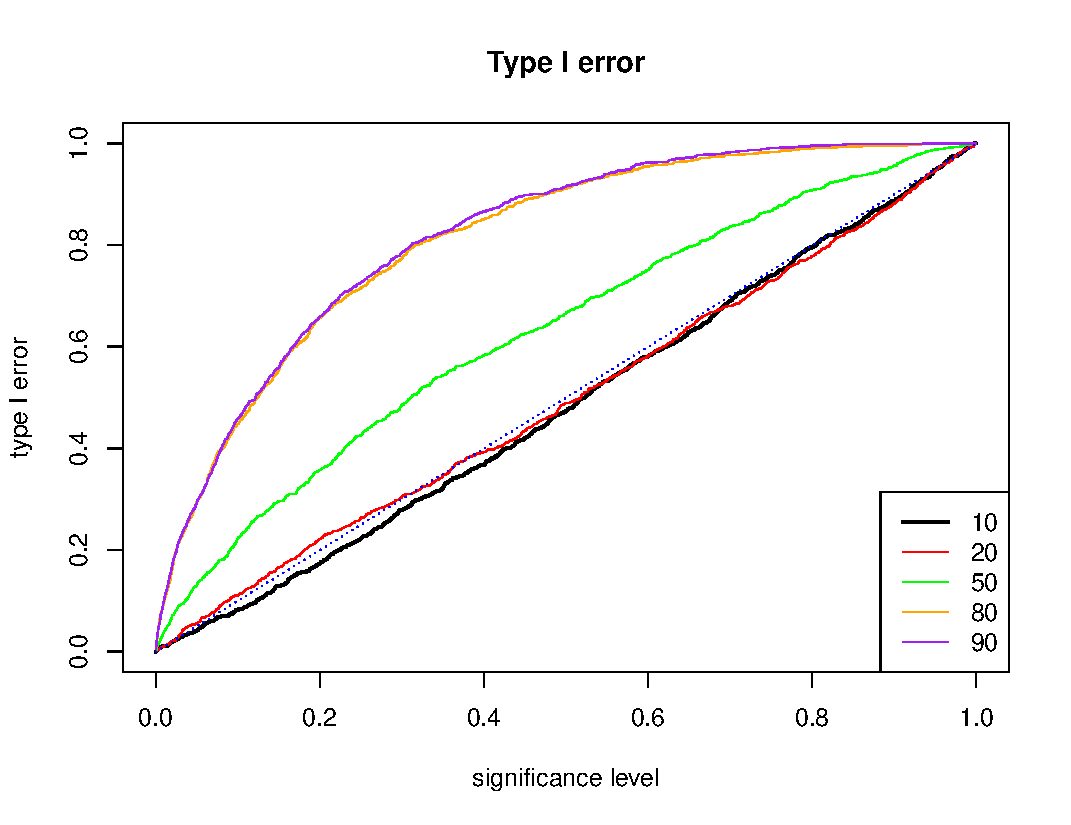
\includegraphics[width=\textwidth]{type1error_sum_ev.pdf}
			\caption{Sum}\label{fig:error_sum}
		\end{subfigure}\hspace{\fill}
		\begin{subfigure}[t]{0.45\textwidth}
			\centering
			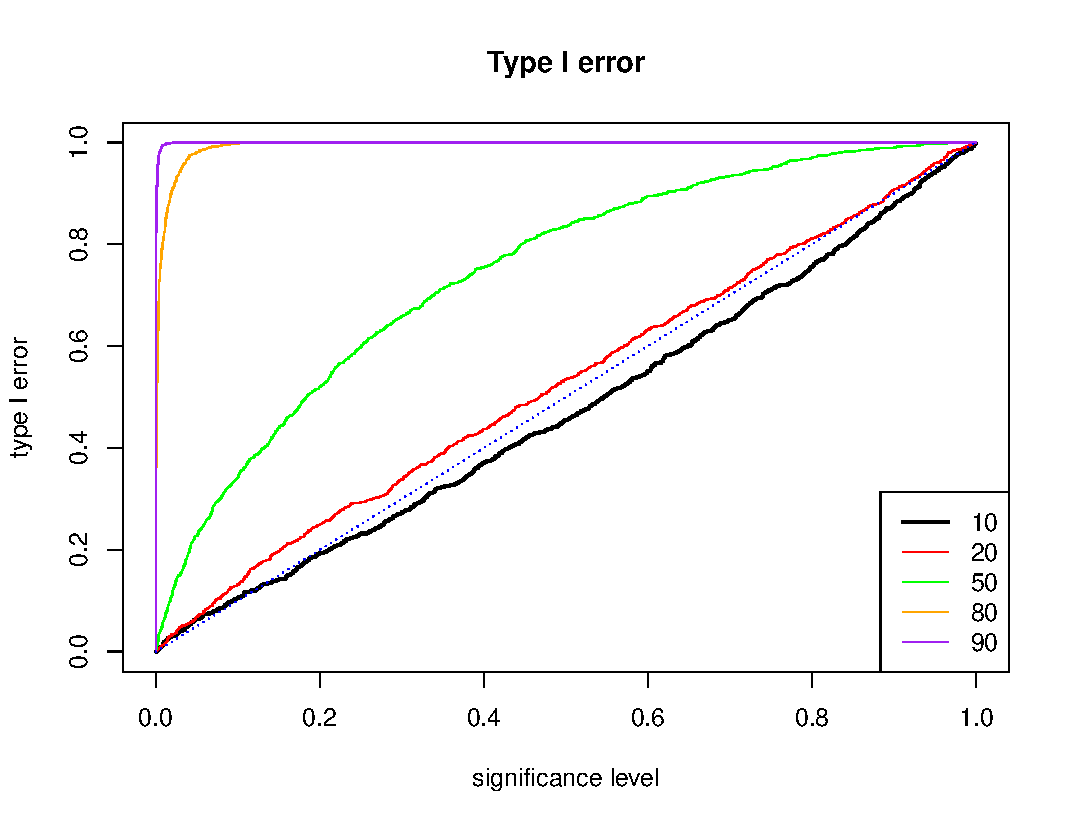
\includegraphics[width=\textwidth]{type1error_mssa_ev.pdf}
			\caption{базовый MSSA}
		\end{subfigure}
		\caption{\textbf{Ошибка первого рода} критерев с проекцией на левые векторы методов Sum и базового MSSA.}
	\end{figure}
	\note{
	На данном графике представлен график ошибки первого рода критериев с проекцией на левые векторы. Слева изображен метод Sum, справа "--- Basic MSSA. Видно, что Toeplitz MC-MSSA с методом Sum значительно уменьшил радикальность критерия.
	}
\end{frame}

\begin{frame}{Полученные результаты: MC-MSSA. Численное сравнение методов. Метод Sum. Продолжение.}
	\begin{figure}
		\captionsetup[subfigure]{justification=Centering}
		\begin{subfigure}[t]{0.45\textwidth}
			\centering
			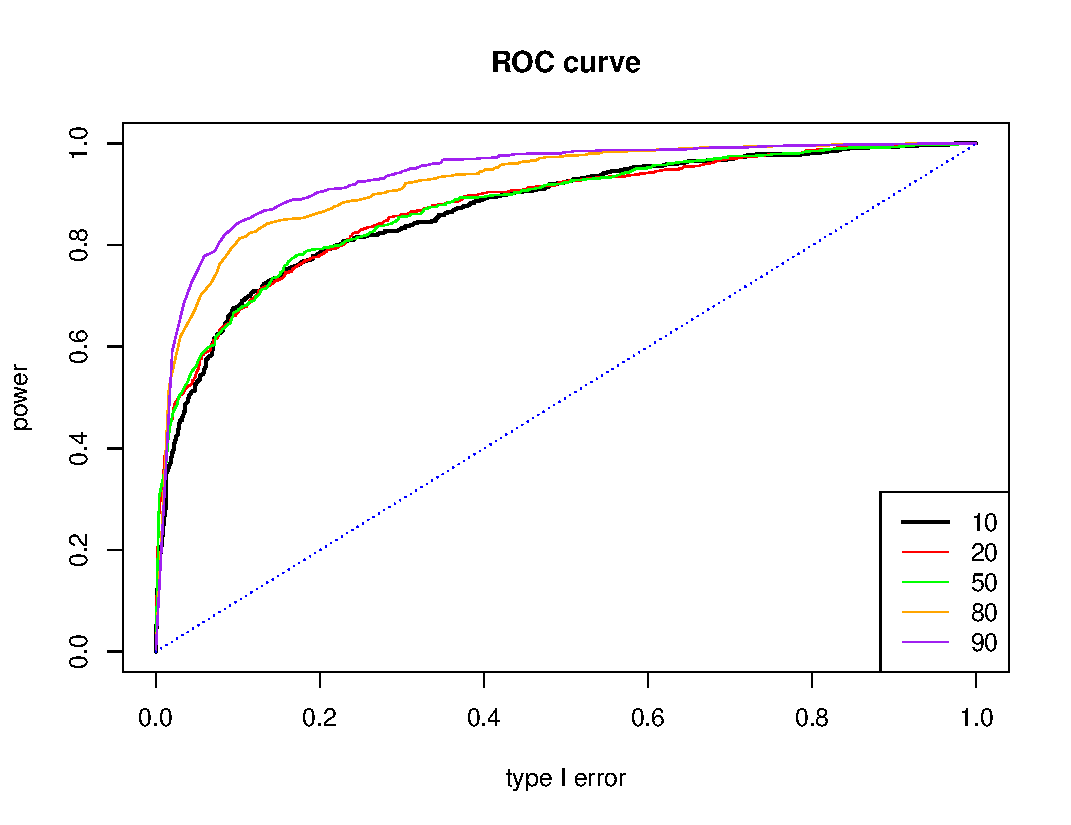
\includegraphics[width=\textwidth]{roc_sum_ev.pdf}
			\caption{Sum}
		\end{subfigure}\hspace{\fill}
		\begin{subfigure}[t]{0.45\textwidth}
			\centering
			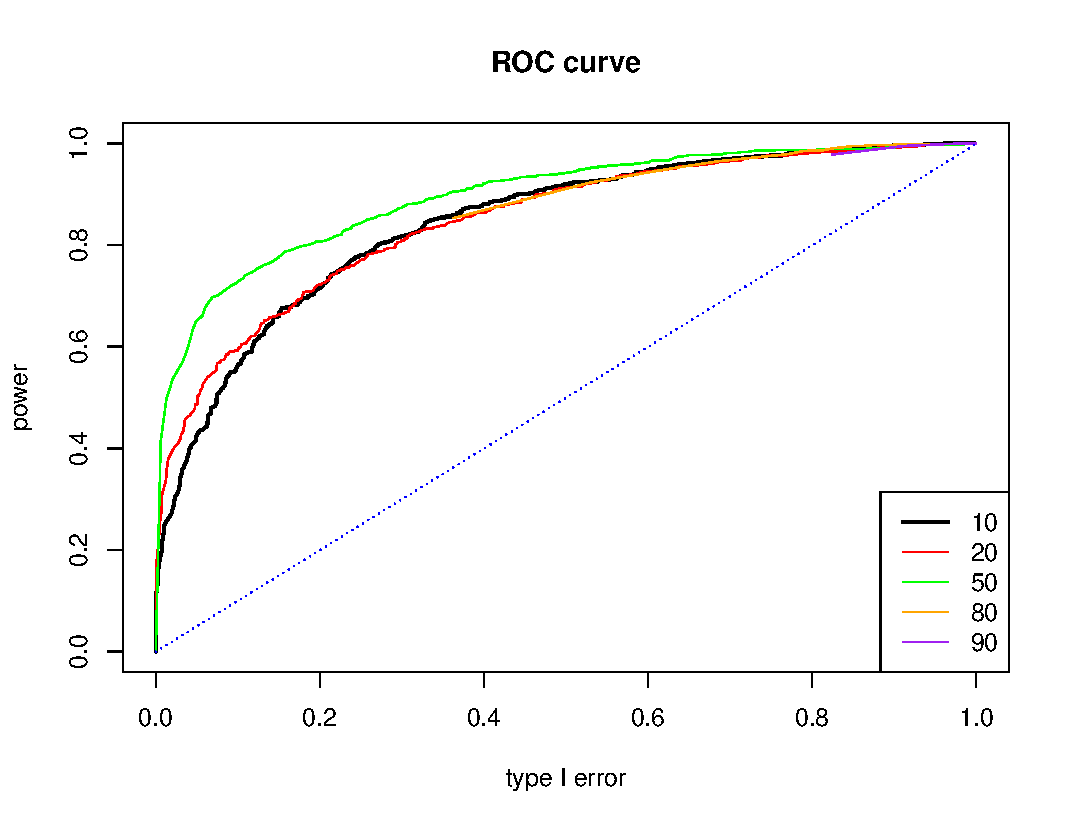
\includegraphics[width=\textwidth]{roc_mssa_ev.pdf}
			\caption{базовый MSSA}
		\end{subfigure}
		\caption{\textbf{ROC-кривая} критериев с проекцией на левые векторы методов Sum и базового MSSA.}
	\end{figure}
	\note{
	Теперь посмотрим на $ROC$-кривые. Слева видим, что наиболее оптимальным значением длины окна является $L=90$, а справа "--- $L=50$. Однако заметим, что из-за очень сильной радикальности, в базовом варианте невозможно было построить ROC-кривые для $L=80$ и $L=90$.
	}
\end{frame}

\begin{frame}{Полученные результаты: MC-MSSA. Численное сравнение методов. Метод Block.}
	\begin{figure}
		\captionsetup[subfigure]{justification=Centering}
		\begin{subfigure}[t]{0.45\textwidth}
			\centering
			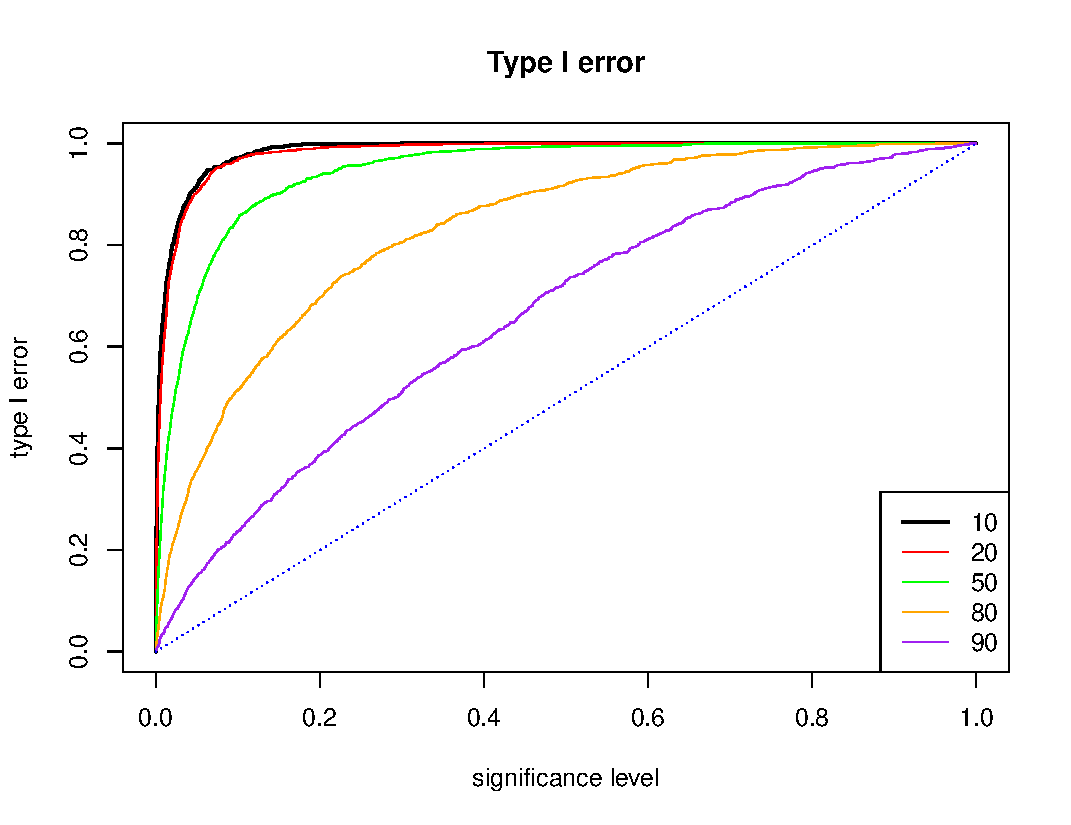
\includegraphics[width=\textwidth]{type1error_block_fa.pdf}
			\caption{Block}
		\end{subfigure}\hspace{\fill}
		\begin{subfigure}[t]{0.45\textwidth}
			\centering
			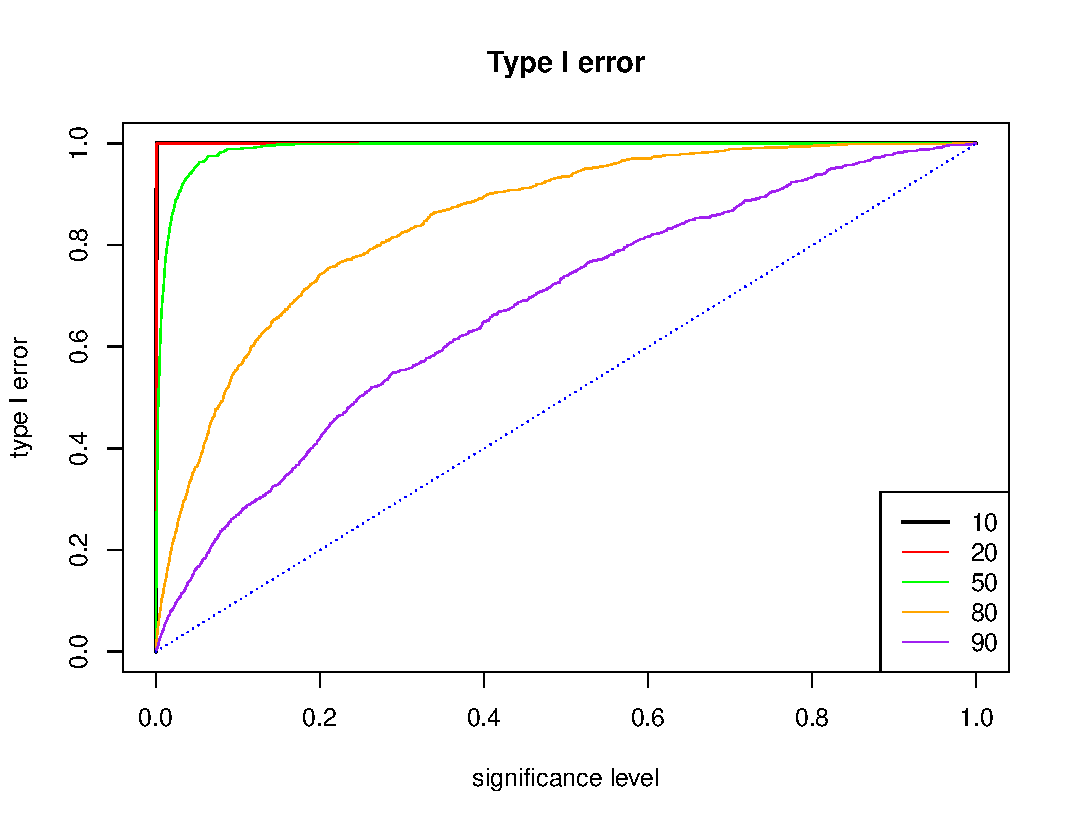
\includegraphics[width=\textwidth]{type1error_mssa_fa.pdf}
			\caption{базовый MSSA}
		\end{subfigure}
		\caption{\textbf{Ошибка первого рода} критериев с проекцией на правые векторы методов Block и базового MSSA.}
	\end{figure}
	\note{
	Сайчас на данном слайде вы наблюдаете график ошибки первого рода критериев с проекцией на правые векторы. Слева изображен метод Block, справа "--- Basic MSSA. В отличие от варианта Sum с проекцией на левые векторы, правые вектора варианта Block дают не настолько заметное снижение радикальности критерия.
	}
\end{frame}

\begin{frame}{Полученные результаты: MC-MSSA. Численное сравнение методов. Метод Block. Продолжение.}
	\begin{figure}
		\captionsetup[subfigure]{justification=Centering}
		\begin{subfigure}[t]{0.45\textwidth}
			\centering
			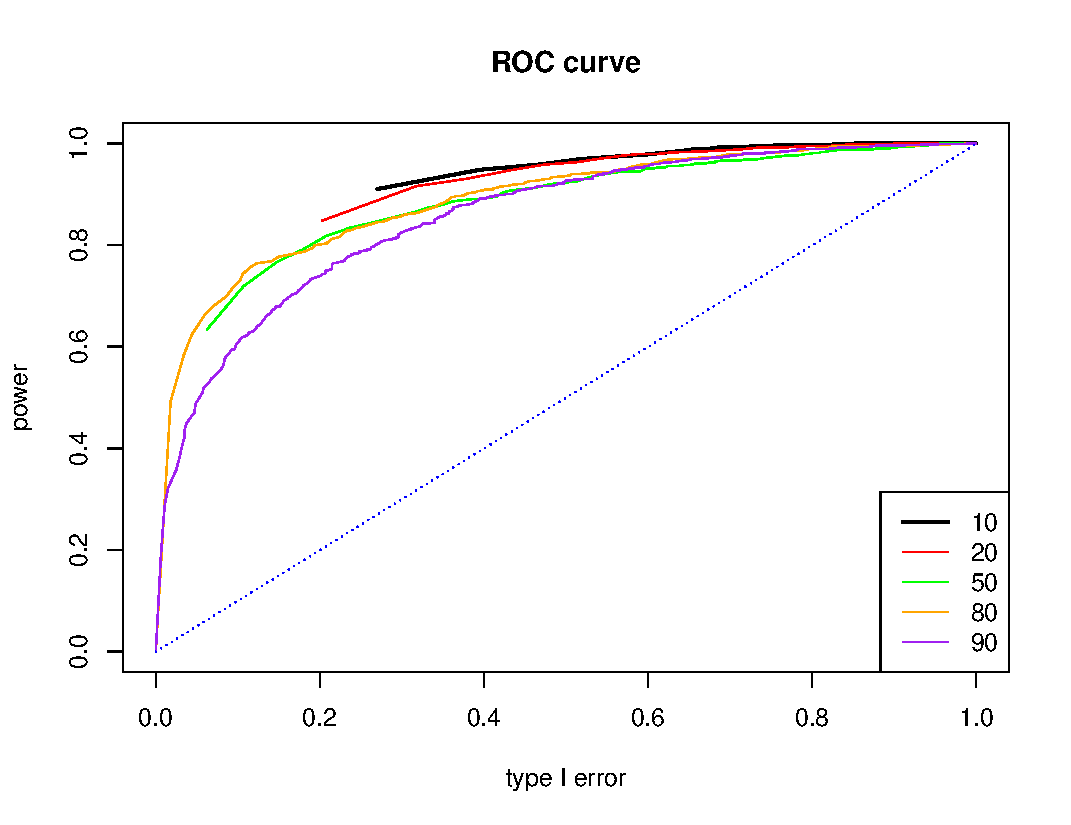
\includegraphics[width=\textwidth]{roc_block_fa.pdf}
			\caption{Block}
		\end{subfigure}\hspace{\fill}
		\begin{subfigure}[t]{0.45\textwidth}
			\centering
			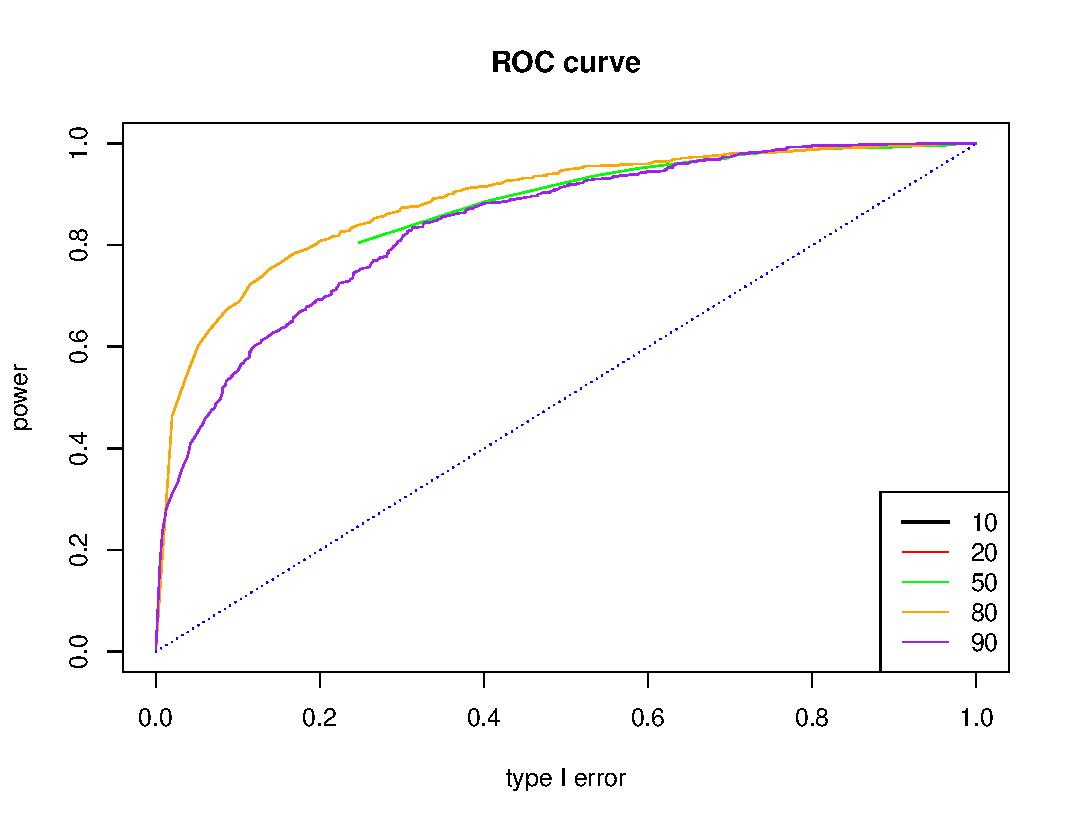
\includegraphics[width=\textwidth]{roc_mssa_fa.pdf}
			\caption{базовый MSSA}
		\end{subfigure}
		\caption{\textbf{ROC-кривая} критериев с проекцией на правые векторы методов Block и базового MSSA.}
	\end{figure}
	\note{
	Напоследок взглянем на ROC-кривые. Для обоих методов наибольшая мощность наблюдается при $L=80$, но из-за слишком большой ошибки первого рода ROC-кривую для $L=10$ и $L=20$, для которых критерий с вариантом Block, предположительно, имеет б\'oльшую мощность, удалось построить не на всем промежутке.
	}
\end{frame}

\begin{frame}{Заключение}
	Мои результаты:
	\begin{enumerate}
		\item Был реализован метод Toeplitz MSSA в вариантах block и sum (на языке $\tR$), на его основе была построена реализация Toeplitz Multiple MC-MSSA.
		\item На основе численных экспериментов были сделаны следующие выводы:
		\begin{itemize}
			\item Sum и Block версии Toeplitz MSSA для стационарного ряда точнее выделяют сигнал, чем Basic MSSA.\vspace{0.25em}
			\item Toeplitz MC-MSSA менее радикален, чем Basic MC-MSSA. Версия Sum с проекцией на собственные вектора оказывается наименее радикальной без потери в мощности скорректированного критерия.
		\end{itemize}
	\end{enumerate}
	В дальнейшем предполагается использовать метод Sum с проекцией на левые векторы, оптимизировать его реализацию и продолжить исследование метода Monte-Carlo MSSA.
	\note{
	В заключение хочу подвести результаты моей работы. Мною был реализован метод Toeplitz MSSA в варинтах Block и Sum на языке программирования $\tR$ и на его основе была построена реализация Toeplitz MC-MSSA.
		
	На основе численных экспериментов были сделаны слелующие выводы: во первых, Sum и Block версии Toeplitz MSSA для стационарного ряда точнее выделяют сигнал, чем Basic MSSA. Если в сигналах разных каналов присутствует одна и та же частота, то Block чуть лучше Sum. Но если частоты разные, то Block существенно хуже Sum.
		
	Во вторых, Toeplitz MC-MSSA менее радикален, чем Basic MC-MSSA. Версия Sum с проекцией на собственные вектора оказывается наименее радикальной без потери в мощности скорректированного критерия.
		
	В дальнейшем предполагается использовать метод Sum с проекцией на левые векторы, оптимизировать его реализацию и продолжить исследование метода Monte-Carlo MSSA. 
	}
\end{frame}

\begin{frame}{Список литературы}
	\begin{thebibliography}{3}
		\bibitem{golyandina2023}
		Golyandina N. Detection of signals by Monte Carlo singular spectrum analysis: multiple testing // Statistics and Its Interface. — 2023. — Vol. 16, no. 1. — P. 147–157.
		\bibitem{larin2022}
		Ларин Е. С. Метод SSA для проверки гипотезы о существовании сигнала во временном ряде : квалификационная работа магистра ; СПбГУ. — 2022.
		\bibitem{golyandina2022}
		Multivariate and 2D Extensions of Singular Spectrum Analysis with the Rssa Package /
		Golyandina Nina, Korobeynikov Anton, Shlemov Alex, and Usevich Konstantin // Journal of Statistical Software. — 2015. — Vol. 67, no. 2.
	\end{thebibliography}
	\note{
	На данном слайде представлен список основных источников, используемых в моей работе.
	}
\end{frame}

\end{document}